%//==============================--@--==============================//%
\clearpage
\subsection[3.4 Interferência intersimbólica]{$\rightarrow$ Interferência intersimbólica}
\label{subsec:intersymbol-interference}

\begin{figure}[H]
    \centering
    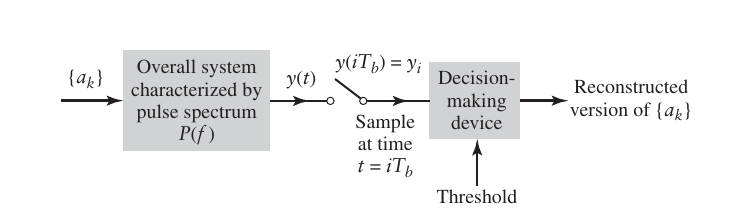
\includegraphics[width = 0.8\linewidth]{img/digital/ISI/Receiver.png}
    \caption{Sistema de receção simplificado.}
    \label{fig:recetor}
\end{figure}

À entrada do \textit{sampler} do esquema do sistema de receção simplificado encontra-se um sinal PAM com pulso $p(t)$ e coeficientes $a_k$ (onde $a_0 = -1$ codifica o bit 0 e $a_1 = +1$ codifica o bit 1):

$$
    x(t) = \sum_{n = -\infty}^{\infty}p(t - n T_b)
$$

\noindent O sinal é amostrado sincronamente com o transmissor:
$$
    x(i T_b) = \sum_{n = -\infty}^p((i - n)T_b)
$$

\noindent Para $n = i$, $p(0) = \sqrt{E}$ (\textit{transmitted signal energy per bit (symbol)}). Onde $n = i$ traduz a sincronia entre i, o instante em que o sinal é amostrado no recetor e n, simbolo do \textit{data stream} produzido pelo transmissor. Isolando o termo para o qual $n = i$ obtemos:

$$
    \boxed{x(i T_b) = a_i\sqrt{E} + \sum_{\substack{n = -\infty\\
                                        n \neq i}}^p((i - n)T_b)}
$$

\noindent A decodificação do símbolo $i$ onde $x_i = \sqrt{E}a_i$ (\textit{perfect decoding}, $a_i$ representa o símbolo binário, com a exceção de um fator multiplicativo) é acompanhada de ruído residual denotado por interferência intersimbólica. A arquitetura do recetor deve ser robusta o suficiente de forma a mitigar/eliminar o ruído adicional.

%//==============================--@--==============================//%
\subsubsection[3.4.1 Critério de Nyquist]{$\rightarrow$ Nyquist Channel}
\label{subsec:NyqCriterion}
O pulso ideal que garante a mitigação da IIS na entrada do \textit{sampler} satisfaz as seguintes duas condições:
$$
    p(t) = \begin{cases}
        1 & t = 0\\
        0 & t \neq 0\\
    \end{cases}
$$

\noindent Amostrando o pulso nos instantes de T: 
$$
    p\delta(t) = \sum_{k = -\infty}^{\infty}p(kT)\delta(t - kT)
$$
\noindent subsequentemente, recorrendo à sua transformanda:
$$
    P\delta(f) = \frac{1}{T}\sum_{k = -\infty}^{\infty}P(f - k/T) = \sum_{k = -\infty}^{\infty}P(kT)e^{-2\pi f T} = p(0) = 1
$$
\clearpage
\noindent Logo podemos admitir que:

$$
    \boxed{P_\delta(f) = \sum_{k = -\infty}^{\infty}P(f - rk) = T}
$$

\noindent Para que que a soma ponto a ponto em $f$ de todas as versões de $P(f)$ transladadas seja constante, garantindo a diminuição de ruído residual é necessário que:

$$
    \boxed{r = 2B_0}
$$

\noindent Onde $B_0$ é a largura de banda fundamental do sinal (\textit{vide} \hyperref[line:unipolarNRZ]{secção sobre \textit{line codes}}, é a largura que alberga a grande maioria da energia do sinal). Supondo um pulso retangular a condição é garantida:

\begin{figure}[H]
    \centering
    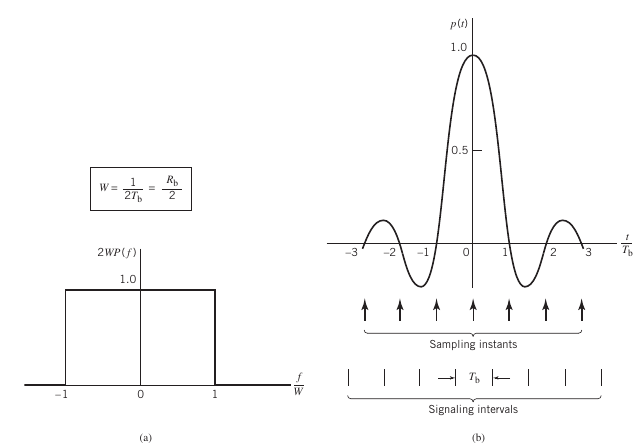
\includegraphics[width = 1\linewidth]{img/digital/ISI/Nyq.png}
    \caption{ (a) Resposta ideal em magnitude. (b) Pulso ideal.}
    \label{fig:Nyq}
\end{figure}

\mdfsetup{linewidth=2pt}
\begin{mdframed}
$\pmb{\star}$ \textbf{Nota:}
\mbox{}\\
Esta relação garante-se apenas para códigos do tipo NRZ, para códigos RZ o pulso dura metade do tempo de bit (símbolo), $r = 2/T$ logo a relação altera-se:
$$
    \boxed{r = B_0}
$$
\noindent Ainda, para um sistema de N níveis (sistemas quaternários, trenários \dots) o \textit{rate} de símbolo relaciona-se com o \textit{rate} de bit da seguinte forma:
$$
\boxed{r_b = \log_2 (M) r_s}
$$
\end{mdframed}
%//==============================--@--==============================//%
\clearpage
\subsubsection[3.4.2 Espetro Raised Cosine]{$\rightarrow$ Espetro Raised Cosine}
\label{subsec:RRC}

``To ensure physical realizability of the overall pulse spectrum $P(f)$, we need a solution that differs from the Nyquist channel in one important respect: the modified $P(f)$ decreases toward zero gradually rather than abruptly. In more specific terms, P1f2 is proposed to consist of two portions:
\begin{enumerate}
    \item Flat portion, which occupies the frequency band $0 \leq |f| \leq f_1$ for some parameter $f_1$ to be defined.
    \item Roll-off portion, which occupies the frequency band $f_1 < |f| < 2B_0  f_1$
\end{enumerate}
For obvious reasons, the $P(f)$ constructed in this manner is called the raised cosine pulse spectrum.''\cite{Haykin2007}
$$
    P(f) = \begin{cases}
            \dfrac{1}{2B_0} & 0 \leq |f| < f_1\\
            \dfrac{1}{4B_0}\left\{1 + \cos(\left[\dfrac{\pi(|f| - f_1)}{2(B_0 - f_1)}\right])\right\} & f_1 \leq |f| < 2B_0 - f_1\\
            0 & 2B_0 - f_1 \leq |f|\\
    \end{cases}
$$

É denominada uma nova variável, \textit{roll-off factor}, relacionada com $f_1$ e $B_0$ da seguinte forma:
$$
    \boxed{\alpha = 1 - \frac{f_1}{B_0}}
$$
\vspace{-1em}
\begin{figure}[ht] 
    \begin{subfigure}[b]{0.5\linewidth}
        \centering
        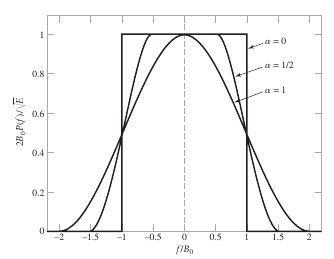
\includegraphics[width=1\linewidth]{img/digital/ISI/MagRRC.png}
        \caption{Espetro RC para vários fatores de \textit{roll-off}.} 
        \label{fig:RRCMag} 
        \vspace{1ex}
    \end{subfigure}%% 
    \begin{subfigure}[b]{0.5\linewidth}
        \centering
        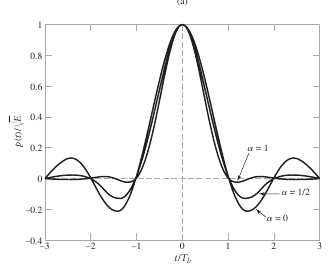
\includegraphics[width=1\linewidth]{img/digital/ISI/TempoRRC.png} 
        \caption{Resposta temporal do pulso.} 
        \label{fig:RRCTempo} 
        \vspace{1ex}
    \end{subfigure} 
    \caption{Pulso Raised Cosine.}
    \label{fig:RRC}
\end{figure}

%//==============================--@--==============================//%
\vspace{-1em}
{
\mdfsetup{linewidth=2pt}

\begin{mdframed}
    $\pmb{\star}$ \textbf{Nota: Transmission Bandwidth Requirement}
    \noindent``(...) The nonzero portion of the raised cosine pulse spectrum P(f) is limited to the interval $(0, 2B_0 - f_1)$ for positive frequencies. Accordingly, the transmission bandwidth required by using the raised cosine pulse spectrum is given by:''\cite{Haykin2007}
    
    $$
        B_t = 2B_0 - f_1 = B_0(1 + \alpha) = \boxed{\dfrac{r_b}{2\log_2(M)}(1 + \alpha)}\qquad (\text{Para códigos NRZ})
    $$

    \noindent Onde $f_v = aB_0$ é a banda adicional (\textit{excess bandwidth}).
\end{mdframed}
}
%//==============================--@--==============================//%
\clearpage
\subsubsection[3.4.3 Eye Pattern]{$\rightarrow$ Eye Pattern}
\label{subsec:EyePattern}

\begin{theo}[\underline{Eye Pattern} \cite{Haykin2007}]{teo/def:nome-unico}\label{teo/def:eyePattern}
    The eye pattern is produced by the synchronized superposition of (as many as possible) successive symbol intervals of the distorted waveform appearing at the output of the receive-filter prior to thresholding.
\end{theo}

\noindent O \textit{Eye Pattern} é uma ferramente de avaliação da qualidade da receção do sinal:
\begin{figure}[H]
    \centering
    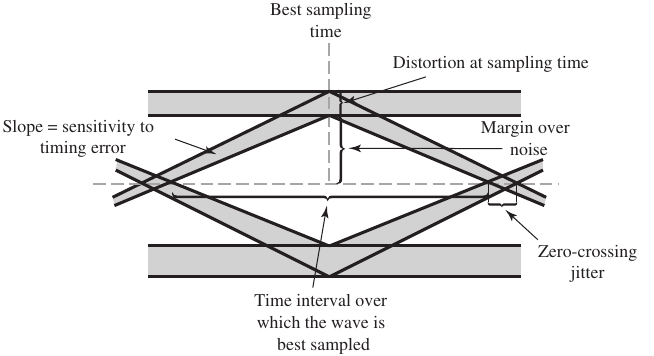
\includegraphics[width = 1\linewidth]{img/digital/ISI/EyePattern.png}
    \caption{Diagrama de Olho.}
    \label{fig:EyePattern}
\end{figure}
%//==============================--@--==============================//%